% !TEX root = ../report.tex


\section{In-vehicle Communication Networks and Security}
\label{sec:communication-networks}

The different functions of a vehicle has very different requirements in
performance and safety needs. Therefor the quality of service needed from the
communication system varies (e.g. response time or bandwidth). Normally there
are different functional domains which divide the in-car embeeded systems
\cite{Navet2017}. There are the safety-critical domains "powertrain" (e.g.
engine control) and "chassis" (e.g. steering) that need a deterministic
real-time behavior. The functions of the "body" domain that controls for example
dashboard, wipers, lights and windows need to exchange many informations of
small size between each other. Other domains like "telematics" and "multimedia"
have increased requirements in for example bandwidth and confidentiality.

TODO: Different networks for different requirements

TODO: Event-triggered versus Time-triggered

\subsection{CAN Network}

\subsection{Time-Triggered Networks}

\subsection{Low-Cost Automotive Networks}

\subsection{Multimedia and Infotainment Networks}

\subsection{Automotive Ethernet}

\subsection{Security Measures}

Controller Authentication, Encrypted Communication, Gateway
Firewalls \cite{Lemke2006}


\section{LeiA: Lightweight Authentication Protocol for CAN}
\label{sec:leia}

Overview of LeiA \cite{Radu2016}


\section{VatiCAN: Vetted, authenticated CAN bus}
\label{sec:vatican}

Overview of vatiCAN \cite{Nurnberger2016}

% \begin{figure}[h]
% 	\centering
% 	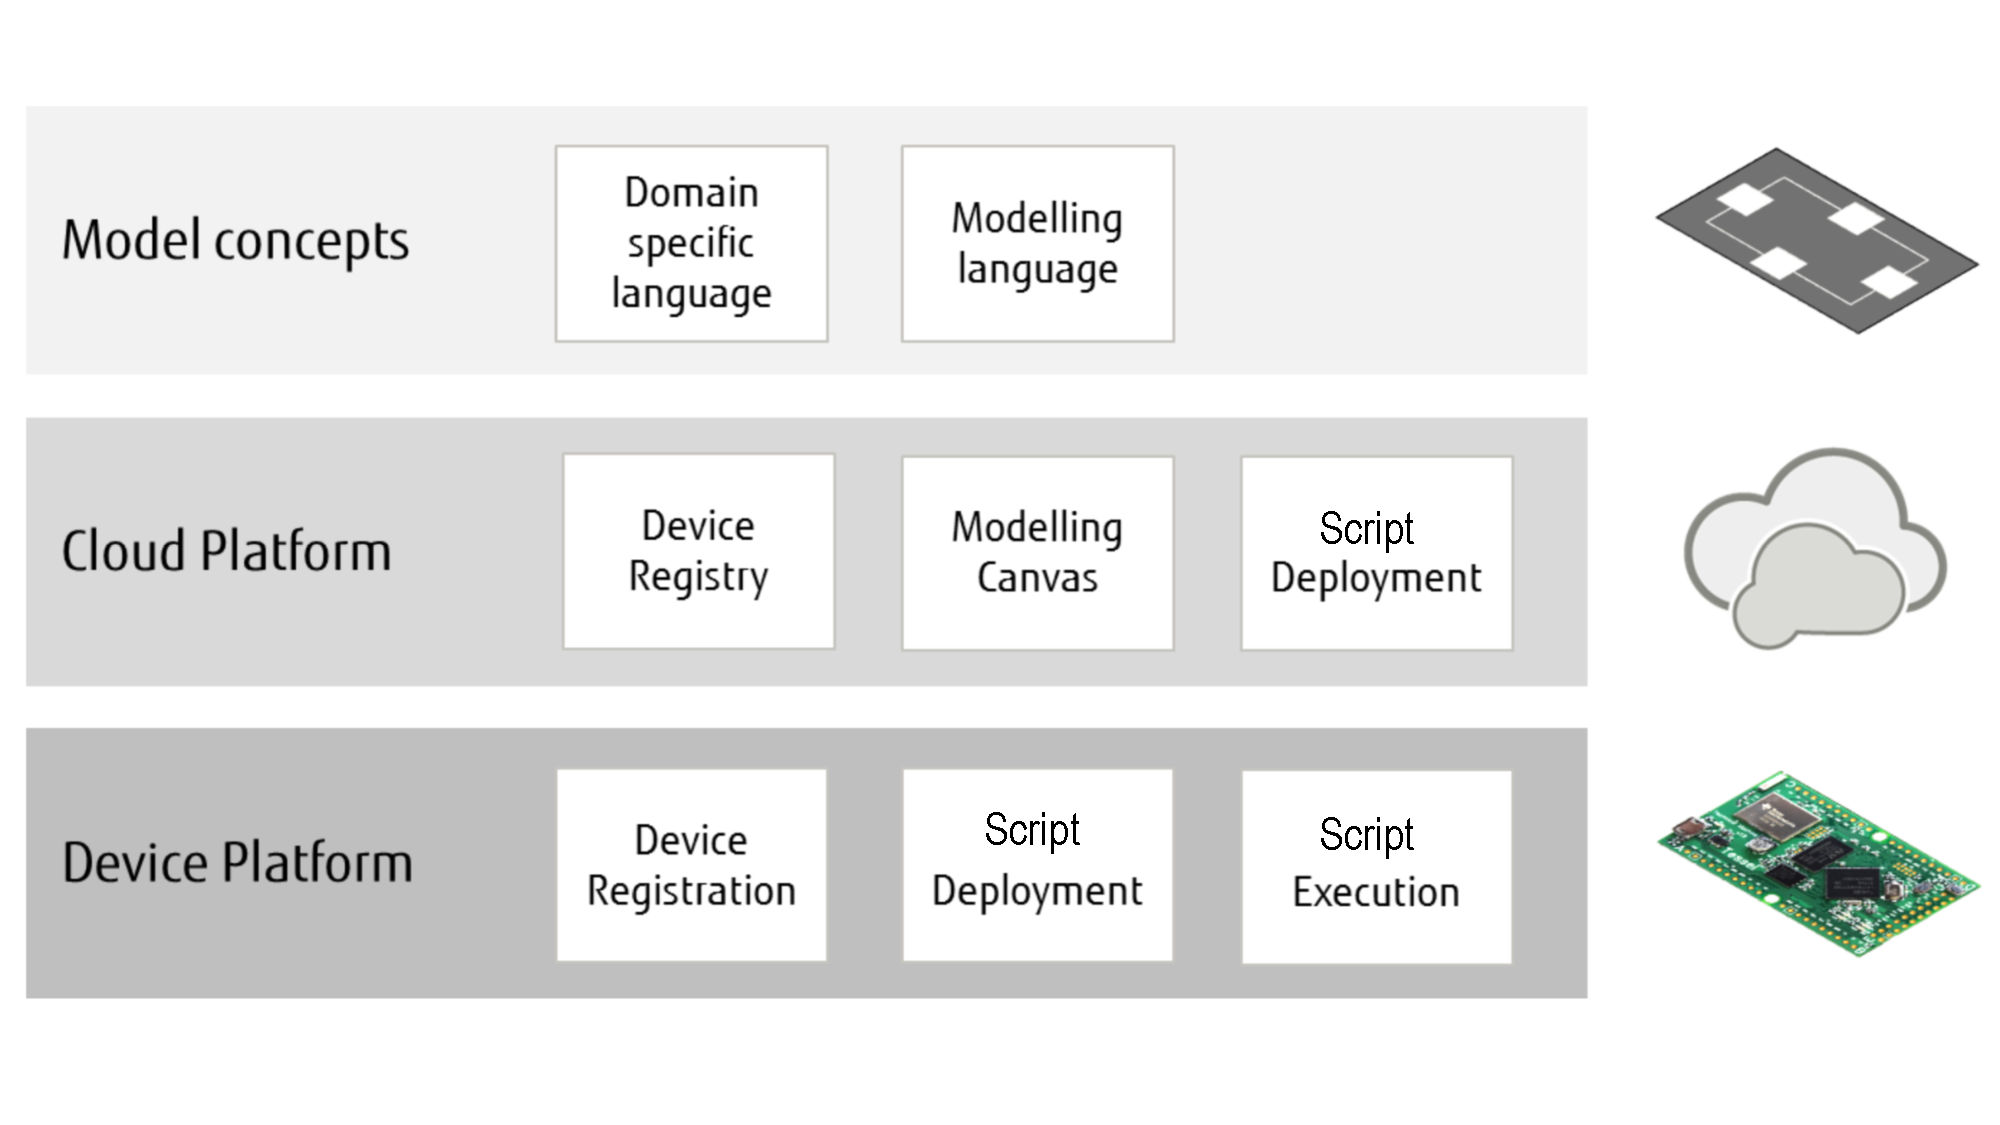
\includegraphics[width=0.8\linewidth]{Figures/sample-figure}
% 	\caption[]{Sample figure.}
% 	\label{fig:sample-figure}
% \end{figure}
